\documentclass{beamer}
\usepackage[english]{babel}
\usepackage{amsmath,amsfonts}
\usepackage{multicol}

\usepackage{IEEEtrantools}
\usepackage{multirow}
% beamer setup

\usetheme{default}
\usecolortheme{seahorse}
%\usecolortheme{dove}

\setbeamertemplate{navigation symbols}{}


\usepackage{tikz}
\usetikzlibrary{shapes,arrows}
\usetikzlibrary{positioning}
\tikzstyle{block} = [rectangle, draw, rounded corners]
\tikzstyle{line} = [draw, -latex']


\DeclareMathOperator*{\argmin}{argmin}
\DeclareMathOperator*{\argmax}{argmax}
\DeclareMathOperator{\E}{\mathbb{E}}
\DeclareMathOperator{\I}{\mathbb{I}}

\AtBeginSection[]{
  \begin{frame}[plain]
  \addtocounter{framenumber}{-1}
  \vfill
  \centering
  %\begin{beamercolorbox}[sep=8pt,center,shadow=true,rounded=true]{title}
    %\usebeamerfont{title}
    \Huge{\insertsectionhead\par}%
  %\end{beamercolorbox}
  \vfill
  \end{frame}
}


\newcommand{\backupbegin}{
   \newcounter{framenumberappendix}
   \setcounter{framenumberappendix}{\value{framenumber}}
}
\newcommand{\backupend}{
   \addtocounter{framenumberappendix}{-\value{framenumber}}
   \addtocounter{framenumber}{\value{framenumberappendix}} 
}




\title{The Economics of Shotgun Marriage}
\subtitle{and Household Bargaining}
\author{Egor Kozlov}

\institute{
  Department of Economics\\
  Northwestern University}
  
  
\setbeamertemplate{footline}[frame number]

  
%  \usepackage{pgf}
%\logo{\pgfputat{\pgfxy(0,0)}{\pgfbox[right,base]{\footnotesize{\insertframenumber\,/\,\inserttotalframenumber}}}}
%\newcommand{\nologo}{\setbeamertemplate{logo}{}}

\begin{document}

\begin{frame}[plain]
\addtocounter{framenumber}{-1}
\date{\scriptsize}
\titlepage
\end{frame}


\begin{frame}%[label=pic0]
\frametitle{In One Picture}
\begin{center}
\includegraphics[width=0.85\linewidth]{diff-by-dt.eps}
\end{center}
%\hyperlink{disc2}{\beamerbutton{dis}}
\end{frame}

\begin{frame}
\frametitle{Shotgun Marriages Perform Worse}
\begin{itemize}
\item Couples who have their kids before marriage divorce more:
\begin{itemize}
\item \textbf{Especially} among college graduates
\item Selection may not be the primary reason
\end{itemize}
\item This teaches us about heterogeneity of marriages:
\begin{itemize}
\item Raising children alone is hard
\item Unplanned pregnancies $\Rightarrow$ lower quality marriages
\item Still important despite access to contraception and abortion
\end{itemize}
\pause
\item \textit{Unexpected pregnancy often triggers marriage}
\item \textit{Unmarried unions with children are rare}
\begin{itemize}
\item \textit{2013: 3\% of children live with unmarried parents}
\item \textit{As opposed to 21\% with single mothers}
\end{itemize}
\end{itemize}
\end{frame}


\begin{frame}
\frametitle{What I Do}

\begin{itemize}
\item Document the fact empirically. Lots of selection!
\item Construct and estimate a structural model 
\item Use it to understand observable differences in divorce rates
\end{itemize}

Main questions:
\begin{itemize}
\item What explains bad performance of shotgun marriage
\item Why college graduates are affected relatively more
\item Role of policies (childcare etc)
\end{itemize}
\end{frame}

\begin{frame}
\frametitle{Main Results}
\begin{itemize}
\item Empirical:
\begin{itemize}
\item Shotgun marriage $\Rightarrow$ divorced $\sim1.8$ more often
\item Among college graduates: $\sim3$ times more often
\item Differences are present after controlling for lots of observables
\item Present is many data sets: ACS, SIPP, NSFG, NSFH
\end{itemize}
\item From the model:
\begin{itemize}
\item Disentangling two main mechanisms:
\begin{itemize}
\item Shotgun marriage couples are different in characteristics
\item Unexpected pregnancy creates large unplanned costs
\end{itemize}
\item Expensive eraly-life childcare explains a lot
\item Higher marginal costs of childcare for skilled women
\item $\sim10\%$ of couples marry because of unplanned pregnancy
\item These couples are the least stable
\end{itemize}
\item Missing pieces (TBD):
\begin{itemize}
\item Quantifying implications
\item Quantifying changes over time
\end{itemize}
\end{itemize}
\end{frame}

\begin{frame}
\frametitle{Implications}
\begin{itemize}
\item Unintended pregnancies $\Rightarrow$ people to pick less favorable partners, ``inefficient'' marriages from ex-ante prospective
\item Child development:
\begin{itemize}
\item Single mothers or blended families $\Rightarrow$ inferior child's outcomes
\item Unstable marriages may be even worse but are often overlooked
\end{itemize}
\item Major impact on women, in particular on:
\begin{itemize}
\item Labor market choices and outcomes
\item Divorces + children worsen re-marriage prospective
\item Total fertility and marriage rates
\end{itemize}
\end{itemize}
\end{frame}

\begin{frame}
\frametitle{Literature}
Shotgun marriages are still a thing:
\begin{itemize}
\item Gibson-Davis et al (2016): 10\% midpregnancy marriages
%\item Akerlof et al (1996)
\end{itemize}
Lifecycle models:
\begin{enumerate}
\item Endogenous bargaining, marriage, divorce \& assets:
\begin{itemize}
\item Voena (2015) --- just divorce, Low et al (2018) --- both
\item Mazzocco (2007) --- seminal paper
\end{itemize}
%\begin{center}
%\textbf{Contribution:} endogenous + exogenous fertility
%\end{center}
\item Fertility:
\begin{itemize}
\item Planned: Sommer (2016)
\item Unplanned: Ejrnæs, Jørgensen (2018)
\end{itemize}
%\begin{center}
%\textbf{Contribution:} bargaining, marriage and divorce
%\end{center}
\item Child investment and marriage/divorce:
\begin{itemize}
\item Lafortune, Low (2018)
\end{itemize}
%\begin{center}
%\textbf{Contribution:} proper lifecycle, fertility
%\end{center}
\end{enumerate}

\textit{Other relevant evidence:}
\begin{itemize}
\item Divorce rates by income: Boertien, Härkönen (2014)
\item Child expenditures by income: Schneider et al (2014)
\end{itemize}
%\item Computations: Judd et al (2014) (thank Luigi Bocola)

\end{frame}

\section{Data Patterns}
\begin{frame}
\frametitle{Pregnancy $\Rightarrow$ Transition Towards Marriage} 
\framesubtitle{NSFH, 2015--2017, weighted frequencies}
\begin{center}
{\Large Before And After Pregnancy}
\begin{tabular}{ l r r r }
 & Single after & Cohabiting after & Married after \\ \hline
\multicolumn{4}{ c }{\textbf{Everyone who gave a birth:}}\\\hline
Single before  & 69.0 & 21.0 & 10.1 \\
Cohabiting before & 4.0 &  74.8 & 21.2 \\
Married before & 0 & 0 & 100 \\\hline
\multicolumn{4}{ c }{\textbf{Ever married only:}}\\\hline
Single before & 56.0 & 22.4 & 21.7 \\
Cohabiting before  & 0.9 & 58.9 & 40.2 \\
Married before & 0 & 0 & 100 \\\hline
\multicolumn{4}{p{0.95\linewidth}}{\small \textit{Note:} this is based on marital status before and after the first reported successful pregnancy.}\\\hline
\hline
\end{tabular}
\end{center}
\end{frame}



\begin{frame}
\frametitle{Definitions: Kids First and Marriage First}
\begin{itemize}
\item Women are units of observation
\item Two groups:
\begin{enumerate}
\item Kids first (\textbf{KF}): youngest child is born before or at the year of marriage. Includes:
\begin{itemize}
\item True shotgun marriages: married when became pregnant
\item Couples who married some time after child's birth 
\item Single mother marrying different partners
\end{itemize}
\item Marriage first (\textbf{MF}): youngest child at least at the next year after marriage
\end{enumerate}
\item Not a full partition
\item Excludes never married
\item Finer partition among KF is available in some datasets
%\item Exclude if more than 5 years before or 10 years after
\end{itemize}
\end{frame}

\begin{frame}[label=disc-sharp]
\frametitle{Sharp Discontinuity in Divorce Rates (Once Again)}
\begin{center}
\includegraphics[width=0.85\linewidth]{diff_dt_h.pdf}
\end{center}
\hyperlink{disc2}{\beamerbutton{controls}}
\end{frame}


\begin{frame}
\frametitle{Composition is Different}
\begin{center}\small
\begin{tabular}{ l c c c c }\cline{2-4}
\multicolumn{1}{c}{} &  \multicolumn{3}{c}{Married once + have kids}\\\cline{2-4}
\multicolumn{1}{c}{}  & Everyone & Kids-first & Marriage-first \\\cline{2-4}\hline
%\textit{Age}     &  33.1     &       31.7     &       33.6 \\
\textit{Age at first marriage}         &   23.3        &    23.6        &    23.2 \\
\textit{Age at first birth}         &     25.4     &       21.7       &     26.5 \\
\textit{Husband's age}         &    35.8      &      34.4   &         36.2  \\
%\textit{Age difference (W$-$H)}        &      2.8      &       3.0      &       2.7  \\\hline
\textit{Eldest child's age}         &    7.8    &        10.0     &        7.1 \\
\textit{Number of children}        &      2.0      &       2.3     &       2.0 \\\hline
\textit{College or + (own), percent}    &         39.5     &       16.9     &       46.3 \\
\textit{College or + (husband), percent}      &       36.4     &       14.2       &     42.7 \\\hline
\textit{In Labor Force, percent}     &        68.6    &        70.0        &    68.2 \\
\textit{Own income, in \$1000}  &         38.4 &          29.1 &         41.1 \\
%\textit{Hours worked}       &     36.5    &        36.8        &    36.4\\
\hline
\textit{White, percent}       &      76.5      &      72.2     &      77.8 \\
\textit{Black, percent}  &        6.7 &            12.2       &       5.0 \\\hline\hline
\multicolumn{4}{p{0.8\linewidth}}{\footnotesize ACS, women, 20--40. Means. Everything is for subsamples when the characteristic is well-defined, for instance, income and hours are for subsample of women who are employed.}\\\hline
\end{tabular}
\end{center}
\end{frame}


\begin{frame}[label=ratios-ACS]
\frametitle{ACS: Shares of Divorced}
\begin{center}
\begin{tabular}{ l  c  c c c | c }\hline
&  \multicolumn{4}{ l|}{\footnotesize{\% of divorced (now), 20--40}} & \\
  & \footnotesize MF & \footnotesize  KF & \footnotesize Ratio & \footnotesize Adjusted &  \scriptsize  \textbf{\% of  KF} \\ \hline
\textit{Everyone} &  \footnotesize 10.1 &  \footnotesize 18.0 & \footnotesize \textbf{1.8} & \footnotesize 1.6 &  \footnotesize 23.2 \\
\textit{35--40} &  \footnotesize 11.3  &  \footnotesize 23.0  & \footnotesize \textbf{2.0} & \footnotesize 1.6 &  \footnotesize 18.0 \\
\textit{High school} &\footnotesize 13.9 & \footnotesize  17.2 &  \footnotesize  \textbf{1.2} & \footnotesize 1.6 & \footnotesize 34.2 \\
\textit{College grads} & \footnotesize 5.3 &  \footnotesize 14.7 &  \footnotesize  \textbf{2.8} & \footnotesize 1.7 &  \footnotesize 9.9 \\\hline
\multicolumn{6}{p{0.8\linewidth}}{\footnotesize ``Adjusted'' refers to corrected for compositions using controls: age, age at 1st marriage, age at 1st birth, education, race, state,  ACS year, number of children}\\\hline\hline
\end{tabular}
\end{center}

\begin{itemize}
\item ACS does not have full marital history, so this is for sample of women who married exactly once 
\item SIPP with full marital history --- same results
\item Income controls --- minor differences, but attrition.
\end{itemize}

\hyperlink{table-ACS}{\beamerbutton{Diff + SE}}
%\hyperlink{pic-ACS}{\beamerbutton{Picture}} 
\hyperlink{table-sipp}{\beamerbutton{SIPP table}} 
\hyperlink{age1b}{\beamerbutton{By age of the first birth}} 
\hyperlink{age1m}{\beamerbutton{By age of the first marriage}}

\end{frame}

\begin{frame}[label=nsfg]
\frametitle{NSFG: The Finest Partition}
Recent data: 2015--2017
\begin{center}
\begin{tabular}{ l  c  c c | c }\hline
\multicolumn{4}{ c |}{Percentage of Divorced, Everyone, 20--40} & \\\hline
 &\footnotesize Percentage & \footnotesize Ratio & \footnotesize Adjusted & \footnotesize \textit{Share}  \\\hline
\footnotesize Marriage First &  24.5 & \textbf{1.00} & 1.00   &  58.8 \\
\footnotesize KF: true shotgun  & 50.7 & \textbf{2.07} & 1.68  & 12.4 \\
\footnotesize KF: before marriage  & 36.8  & \textbf{1.50} & 1.60 & 20.6 \\
\footnotesize KF: new partner & 31.7 & \textbf{1.29} & 1.64 & \phantom{0}8.1  \\\hline
\multicolumn{4}{p{0.7\linewidth}}{\footnotesize ``Adjusted'' refers to corrected for compositions using controls: age, age at 1st marriage, age at 1st birth, education, race, number of children}\\\hline\hline
\end{tabular}
\end{center}
\end{frame}



\begin{frame}[label=hazards]
\frametitle{NSFH: Hazards of Divorce}
Historical Data: average 40 years old at 1987
\begin{center}
\begin{tabular}{ l  c  c c c }\hline
\multicolumn{5}{ c }{Cox Regression: Hazard Ratios (S.E.)}\\\hline
 &\footnotesize Everyone & \footnotesize Everyone & \footnotesize Non-college & \footnotesize  College \\\hline
\footnotesize all KF & \footnotesize 1.45 (0.12) & --- &\footnotesize  1.45 (0.15) &\footnotesize  2.23 (0.81)  \\ 
\footnotesize true shotgun  & --- &\footnotesize  1.34 (0.12) & --- & --- \\
\footnotesize before marriage  & --- & \footnotesize  2.18 (0.28) & --- & ---  \\\hline\hline
\multicolumn{5}{p{0.9\linewidth}}{\footnotesize controls: age, age at 1st marriage, age at 1st birth, education, race, number of children}\\\hline\hline
\end{tabular}
\end{center}
\end{frame}



\begin{frame}
\frametitle{More Evidence}
\begin{enumerate}
\item Divorce rates start being different when the eldest child is 5--10 years old
\item Comparing marriages of the same duration exacerbates the difference
\item NLSY, Cox duration model: 2.3 times more likely to divorce if same-year (thank Fabio Blasutto)
\item Children in KF couples repeat grades more often
\end{enumerate}
\end{frame}



\section{Model Features}

\begin{frame}
\frametitle{Overview}
\begin{itemize}
\item Lifecycle model
\item Assets ($a$) and productivity shocks ($z^f$, $z^m$)
\item Endogenous marriage and divorce (limited commitment)
\item Reduced form marriage market:
\[p^{\text{meet}}(\text{Age}) \text{ --- meeting a random partner with similar $a$ and $z$}\]
\item Both endogenous and unplanned fertility:
\[p^{\text{unplanned}}(\text{Age},z^f) \text{ --- arrival of unplanned kids}\]
\end{itemize}
\end{frame}

\begin{frame}
\frametitle{Modeling Shotgun Marriage}
\begin{center}
\vspace{-0.75cm}
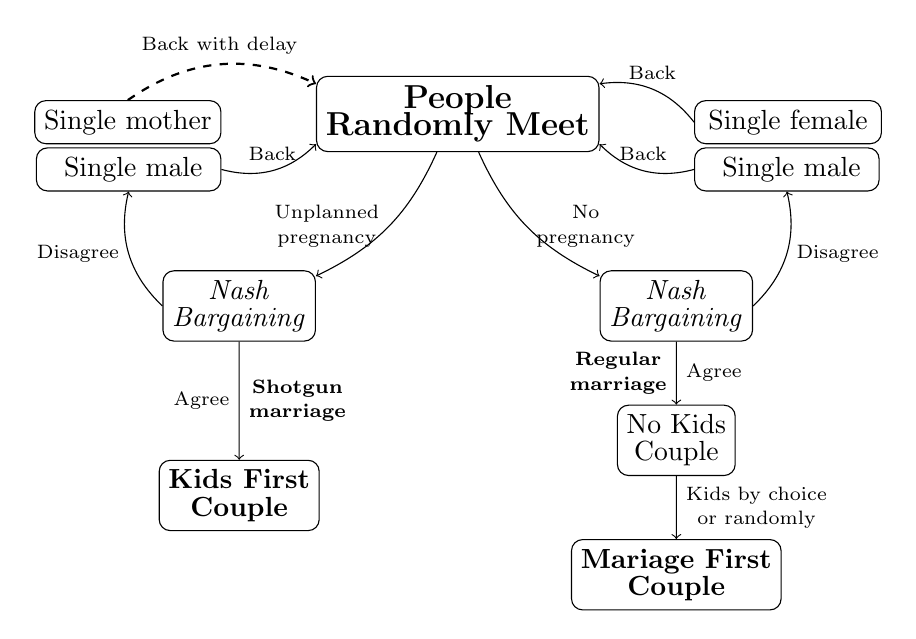
\begin{tikzpicture}[every text node part/.style={align=center}, scale=0.75]
   % Place nodes
   \node [block] (1) {\large \textbf{People}  \\[-0.5ex]  \large  \textbf{Randomly Meet}};
   \node [block, below left = 1.5 cm and 0.0 cm of 1] (2) {\textit{Nash} \\[-0.5ex] \textit{Bargaining}};   
   \node [block, below right = 1.5 cm and 0.0 cm of 1] (3) {\textit{Nash} \\[-0.5ex] \textit{Bargaining}};   

   \node [block, below = 1.5 cm of 2] (5) {\textbf{Kids First} \\[-0.5ex] \textbf{Couple}};
   \node [block, below = 0.8 cm of 3] (7) {No Kids \\[-0.5ex] Couple};
   \node [block, below = 0.8 cm of 7] (8) {\textbf{Mariage First} \\[-0.5ex] \textbf{Couple}};
   \draw[->] (1) to [bend left = 20] node [left] {\scriptsize Unplanned \\[-0.75ex] \scriptsize pregnancy} (2);
   \draw[->] (1) to [bend right = 20] node [right] {\scriptsize No \\[-0.75ex] \scriptsize pregnancy} (3);
   \draw[->] (2) to node [left] {\scriptsize Agree} node [right] {\scriptsize \textbf{Shotgun} \\[-0.75ex]  \scriptsize \textbf{marriage}} (5);
   \draw[->] (3) to node [right] {\scriptsize Agree} node [left]  {\scriptsize \textbf{Regular} \\[-0.75ex]  \scriptsize \textbf{marriage}} (7);
   \draw[->] (7) to node [right] {\scriptsize Kids by choice \\[-0.75ex] \scriptsize or randomly} (8);   

\pause  
  
    \node [block, above left   = 1.0 cm and -0.75 cm of 2] (4) {\,\, Single male\,\,};
    \node [block, above left   = 1.6 cm and -0.75 cm of 2] (4-sm) {Single mother};
	\node [block, above right   = 1.0 cm and -0.75 cm of 3] (6) {\,\, Single male\,\,};
    \node [block, above right   = 1.6 cm and -0.75 cm of 3] (6-f) {\,Single female\,};   
    \draw[->] (2.180) to [bend left = 30] node [left] {\scriptsize Disagree} (4.270);
    \draw[->] (3.0) to [bend right = 30] node [right] {\scriptsize Disagree} (6.270);
     \draw[->] (6.180) to [bend left = 30] node [above] {\scriptsize Back}  (1.-12);
   \draw[->] (6-f.180) to [bend right = 30] node [above] {\scriptsize Back} (1.12);
   \draw[->,thick,dashed] (4-sm.90) to [bend left = 30] node [above] {\scriptsize Back with delay}  (1.168);
   \draw[->] (4.0) to [bend right = 30] node [above] {\scriptsize Back} (1.192);
   
   
\end{tikzpicture}
\end{center}
\end{frame}

\begin{frame}[label=utilities]
\frametitle{Utility Functions}
\begin{itemize}
\item Couple, $\theta$ --- Pareto weight, $\psi$ --- common love shock:
\[U = \theta \cdot u(c_f) + (1-\theta)\cdot u(c_m) + \psi,\]
\item Couple + child, $Q$ --- child quality (public good):
\[U = \theta \cdot \tilde{u}(c_f,Q) + (1-\theta)\cdot \tilde{u}(c_m,Q) + \psi,\]
\item Child quality: $Q = F(x,l^f)$, $x$ --- money, $l^f$ --- female time
\item Budget constraint ($C$ reflects returns to scale, $a$ --- assets):
 \[C(c_f,c_m) + a' + x = R\cdot a + (1-l^f)\cdot W^f_t(z_f) + W^m_t(z_m),\]
\end{itemize}
\hyperlink{value-functions}{\beamerbutton{Value Functions}}
\end{frame}


\begin{frame}
\frametitle{Marriage}
\begin{itemize}
\item People (f \& m) meet, get a draw of love shock $\psi$ and agree to marry if exists a Pareto weight $\theta$ such that
\[V^{f,\text{yes}}(\underset{\scriptsize +}{\theta\vphantom{\psi}},\underset{\scriptsize +}{\psi}) \geq V^{f,\text{no}}, \ \ \ \ V^{m,\text{yes}}(\underset{\scriptsize  -}{\theta\vphantom{\psi}},\underset{\scriptsize +}{\psi}) \geq V^{m,\text{no}}.\]
\item Young children require lots of female time
\item \textbf{Mechanism:} unplanned pregnancy 
\begin{enumerate}
\item[(1)] lowers current $V^{f,\text{no}}$: hard to be a single mother
\item[(2)] increases future $V^{m,\text{yes}}$ and $V^{f,\text{yes}}$: good to have children
\end{enumerate} 
$(1) + (2)$ $\Rightarrow$ the couple agrees to marry with lower $\psi$ and $\theta$.
\end{itemize}
\end{frame}

\begin{frame}
\frametitle{Divorce}
\begin{itemize}
\item Shocks to $\psi$, $z^f$ and $z^m$
\item People cannot commit not to divorce
\item $\theta$ may be renegotiated, stays constant if not
\item Divorce happens if no $\theta$ exist such that
\[V^{f,\text{together}}(\theta,\psi) \geq V^{f,\text{divorce}}, \ \ \ \ V^{m,\text{togetehr}}(\theta,\psi) \geq V^{m,\text{divorce}}.\]
\item Couples with lower $\psi$ or more unequal $z$ divorce more!
\item As children get older they require less time
\end{itemize}
\end{frame}


\section{Fit and Results}
\begin{frame}
\frametitle{Strategy}
\begin{itemize}
\item I use Simulated Method of Moments to calibrate $\sim 16$ parameters:
\begin{itemize}
\item Preferences
\item Probabilities of transitions
\item Child quality technology
\end{itemize}
\item Income paths to match ACS
\item The target moments are taken from:
\begin{itemize}
\item ACS (raw divorce, fertility and marriage shares by groups)
\item CEX + ATUS (time and money spent on childcare)
\end{itemize}
\end{itemize}
\end{frame}

\begin{frame}
\frametitle{Targeted Moments}
\begin{tabular}{ l r r}\hline
Target & Model & Data \\\hline
\footnotesize\textit{Never married by (25,35,40), \% }& $(61,25,19)$ &  $(68,26,19)$ \\
\footnotesize \textit{One marriage by 40, \%}  & $70$ & $65$ \\\hline
\footnotesize \textit{No children by (25,35,40), \%}  & $(65,27,24)$ & $(67,28,26)$ \\
\footnotesize \textit{... by 30 (low-$z$,high-$z$), \%}  & $(52,57)$ & $(44,58)$ \\\hline
\footnotesize \textit{Divorced by (25,35,40), \%}  & $(5,11,16)$ & $(11,16,19)$ \\
\footnotesize \textit{... by 30 (low-$z$,high-$z$), \%}  & $(17,9)$ & $(21,8)$ \\\hline
\footnotesize \textit{Divorced by (30,35,40), \%}  & $(5,11,16)$ & $(11,16,19)$ \\
\footnotesize \textit{... by 40 (KF,MF), \%}  & $(25,15)$ & $(24,13)$ \\\hline
\footnotesize \textit{Money for childcare ($\%$ tot expend)} & $43.4$ & 40.0 \\
\footnotesize \textit{Time spent low-$z$/high-$z$ (ratio)} & 1.11 & 1.19 \\
\footnotesize \textit{Money spent low-$z$/high-$z$ (ratio)} & 2.56  & 2.67 \\\hline

\end{tabular}
\end{frame}


\begin{frame}
\frametitle{Model Allows for Eliminating Selection}

\begin{itemize}
\item Generate $5{,}000$ individuals from unconditional distribution
\item No one meets partners till 25.
\item At 25, two scenarios. All of them:
\begin{itemize}
\item Meet and become pregnant --- KF if agree
\item Meet and do not become pregnant --- MF if agree
\end{itemize}
\item Look at their outcomes over time
\end{itemize}
\end{frame}

\begin{frame}
\frametitle{Causal Impact $\approx$ Observable Impact}
\begin{center}
\includegraphics[width=0.85\linewidth]{../main/individual-av.eps}
\end{center}
\end{frame}



\begin{frame}
\frametitle{Lower Child Investment Even without Selection2}
\vspace{-2cm}
\begin{center}
\includegraphics[width=1.0\linewidth]{../main/x-time.pdf}
\end{center}
\end{frame}


\begin{frame}
\frametitle{``Compliers'' Drive Everything}
\begin{center}
\includegraphics[width=0.85\linewidth]{../main/ind-decomp.eps}
\end{center}
\end{frame}

\newcommand{\pz}{\phantom{0}}
\begin{frame}
\frametitle{More Impact In Early Life}
\begin{center}
\begin{tabular}{ l c c c}\hline 
& &  \multicolumn{2}{ c }{\scriptsize  No Unplanned Pregnancies}  \\
& \scriptsize Baseline & \scriptsize Outside Marriage & \scriptsize At all \\\hline
\footnotesize Divorced by 25, \% & $\pz4.5$   & $\pz3.2$ & $\pz2.3$ \\
\footnotesize Divorced by 30 (low-$z$), \%  & $17.2$ & $14.6$   & $11.9$ \\
\footnotesize Divorced by 30 (high-$z$), \%  & $\pz9.0$ & $\pz8.2$  &  $\pz7.4$ \\
\footnotesize Divorced by 35, \%  & $10.8$  & $\pz9.9$&   $\pz9.2$  \\
\footnotesize Divorced by 40, \%  & $16.3$ & $15.4$ &  $14.8$ \\\hline
\end{tabular}
\end{center}
\end{frame}

\begin{frame}
\frametitle{Conclusions And Plans}
\begin{itemize}
\item What we observe about childcare costs generates the pattern
\item KF couples have lower $\psi$ and divorce more
\item Unplanned pregnancies account for $1/2$ of early-age divorces
\item Preparing a new iteration now:
\begin{itemize}
\item TBD: partition by income needs to be improved
\item TBD: decompose by different contributors ($z$, $\psi$, age)
\end{itemize}
\item Model allows to account for other stories:
\begin{itemize}
\item Labor market discrimination of unmarried mothers
\item Social stigma against unmarried cohabitation
\item ...
\end{itemize}
\end{itemize}



\end{frame}



\backupbegin

\appendix
\section{Appendix}



\begin{frame}[label=table-ACS]
\frametitle{Slicing and Adding Controls}
\begin{center}
\begin{tabular}{ l  c  c c c | c }\hline
&  \multicolumn{4}{ l|}{\footnotesize{\% of divorced (now), 20--40}} & \\
  & \footnotesize MF & \footnotesize  KF & \footnotesize Diff / (s.e.) & \footnotesize Diff w/controls${}^*$ &  \scriptsize  \textbf{\% of  KF} \\ \hline
\textit{Everyone} &  \footnotesize10.1 &  \footnotesize 18.0 & \footnotesize \textbf{\phantom{0}7.9 / (0.1)} & \footnotesize 5.7 / (0.2) &  \footnotesize 23.2 \\
\textit{35--40} &  \footnotesize 11.3  &  \footnotesize 23.0  & \footnotesize \textbf{11.7 / (0.1)} & \footnotesize 6.7 / (0.3) &  \footnotesize 18.0 \\
\textit{High school} &\footnotesize 13.9 & \footnotesize  17.2 &  \footnotesize  \textbf{\phantom{0}3.3 / (0.2) }& \footnotesize 8.4 / (0.3) & \footnotesize 34.2 \\
\textit{College grads} & \footnotesize 5.3 &  \footnotesize 14.7 &  \footnotesize  \textbf{\phantom{0}9.4 / (0.2) }& \footnotesize 3.8 / (0.3) &  \footnotesize 9.9 \\\hline
\multicolumn{6}{p{0.9\linewidth}}{\footnotesize ${}^*$ controls include: age, age at 1st marriage, age at 1st birth, race, state, ACS year, number of children}\\\hline\hline
\end{tabular}
\end{center}



\hyperlink{ratios-ACS}{\beamerbutton{back}} 
\hyperlink{pic-ACS}{\beamerbutton{Picture}} 
\hyperlink{table-sipp}{\beamerbutton{SIPP table}} 
\hyperlink{age1b}{\beamerbutton{By age of the first birth}} 
\hyperlink{age1m}{\beamerbutton{By age of the first marriage}}
\end{frame}


\begin{frame}[label=pic-ACS]
\begin{center}
\includegraphics[width=1.0\linewidth]{../main/shrs.eps}
\end{center}
\hyperlink{table-ACS}{\beamerbutton{back}}
\end{frame}





\begin{frame}[label=table-sipp]
\frametitle{SIPP}
\framesubtitle{Now with full marital history}
\begin{center}
\begin{tabular}{ l  c  c c c | c }\hline
&  \multicolumn{4}{ l|}{\footnotesize{\% of divorced (ever) among women of 20--40}} & \\
  & \footnotesize MF & \footnotesize  KF & \footnotesize Diff / (s.e.) & \footnotesize Diff w/controls${}^*$ &  \scriptsize  \textbf{\% of  KF} \\ \hline
\textit{Everyone} &  \footnotesize 21.1 &  \footnotesize 32.0 & \footnotesize \textbf{10.9 / (0.6)} & \footnotesize 10.4 / (0.8) &\footnotesize 22.8 \\
\textit{35--40} &  \footnotesize 24.5 &  \footnotesize 44.1 & \footnotesize \textbf{19.6 / (1.0)} & \footnotesize 12.4 / (1.4) &\footnotesize 18.9 \\
\textit{High school} &\footnotesize 26.6  &\footnotesize 30.2 &\footnotesize \textbf{\phantom{0}3.6 / (0.9) }& \footnotesize 14.5 / (1.4) &\footnotesize 33.3\\
\textit{College grads} & \footnotesize 11.7  & \footnotesize26.9 &\footnotesize \textbf{15.2 / (1.3)} & \footnotesize 11.5 / (1.4) &\footnotesize 9.5 \\\hline
\multicolumn{6}{p{0.9\linewidth}}{\footnotesize ${}^*$ controls include: age, age at 1st marriage, age at 1st birth, race, state, number of children}\\\hline\hline
\end{tabular}
\end{center}
\begin{itemize}
\item Drawback: smaller sample size 
\end{itemize}
\hyperlink{table-ACS}{\beamerbutton{back}}
\end{frame}



\begin{frame}[label=disc2]
\frametitle{Discontinuity is Still Here}
\begin{center}
\includegraphics[width=0.85\linewidth]{diff-by-dt-con.eps}
\end{center}
\hyperlink{disc-sharp}{\beamerbutton{back}}
\end{frame}




\begin{frame}[label=age1b]
\frametitle{By age of 1st birth}
\begin{center}
\includegraphics[width=0.8\linewidth]{joint-reg-by-age1b.eps}
\end{center}
\hyperlink{age1b-con}{\beamerbutton{controls}}
\hyperlink{table-ACS}{\beamerbutton{back}}
\end{frame}

\begin{frame}[label=age1b-con]
\frametitle{By age of 1st birth + controls}
\begin{center}
\includegraphics[width=0.8\linewidth]{joint-reg-by-age1b-con.eps}
\end{center}
\hyperlink{table-ACS}{\beamerbutton{back}}
\end{frame}


\begin{frame}[label=age1m]
\frametitle{By age of 1st marriage}
\begin{center}
\includegraphics[width=0.8\linewidth]{joint-reg-by-age1m.eps}
\end{center}
\hyperlink{age1m-con}{\beamerbutton{controls}}
\hyperlink{table-ACS}{\beamerbutton{back}}
\end{frame}

\begin{frame}[label=age1m-con]
\frametitle{By age of 1st marriage + controls}
\begin{center}
\includegraphics[width=0.8\linewidth]{joint-reg-by-age1m-con.eps}
\end{center}
\hyperlink{table-ACS}{\beamerbutton{back}}
\end{frame}





\begin{frame}[label=value-functions]
\frametitle{Value Functions --- 1}
\framesubtitle{Single Female}
{\scriptsize
\begin{align}V^{f,s}_t(\omega) = \max\limits_{c} & \bigg\{ u(c) + \beta \E_t \Big[ (1 - p^{\text{meet}}_t)\cdot V^{f,s}_{t+1}(\omega') + \nonumber \\  \nonumber
& \hspace{7em} p^{\text{meet}}_t (1-p^{\text{preg}}_t) \big\{ m^{np} \cdot V^{f,c}_{t+1}(\Omega^c) + (1-m^{np})V^{f,s}_t(\omega')\big\} + \\  \nonumber
& \hspace{10em} p^{\text{meet}}_t p^{\text{preg}}_t \big\{ m^{p} \cdot V^{f,ck}_{t+1}(\Omega^c) + (1-m^{p})V^{f,sk}_{t+1}(\omega')\big\}  \Big]  \bigg\},
\end{align}\vspace{-3em}
\begin{align*}
 \text{s.t. \ }  &  a' = R\cdot a  + W^f_t(z) - c  & \text{ (evolution of assets)}\\
 &  z' = z + \varepsilon^{z,f}_t, \ \ \varepsilon^{z,f}_t \sim \mathcal{N}(0;\sigma_{z,f}^2) &  \text{ (evolution of productivity)}\\
  & \log W^f_t = z_t + \text{Trend}^f_t, \ \ \  \text{Trend}^f_t = a^f_0 + a^f_1\cdot t  +  a^f_2 \cdot t^2 &  \text{ (labor income and trend)}\\
  & \Omega^c = \mathcal{M}^f(a',z') &  \text{ (marriage prospectives)}
\end{align*}
}
\hyperlink{utilities}{\beamerbutton{back}}
\end{frame}


\begin{frame}[label=value-functions]
\frametitle{Value Functions --- 2}
\framesubtitle{Couple, No Children}
{\scriptsize
\begin{align}& \hspace{5em}  V^{c}_t(\Omega) = \max\limits_{c^f,c^m}  \bigg\{ \theta\cdot u(c^f) + (1-\theta)\cdot u(c^m) + \psi + \nonumber \\   \nonumber
 &  \beta \E_t \Big[   (1 - p^{\text{preg}}_t)\cdot \left\{ (1-d^{\text{np}})\cdot \max\left\{ V^{ck}_{t+1},V^{c}_{t+1}\right\} + d^{\text{np}}\cdot [ \theta V_{t+1}^{f,s} + (1-\theta)V_{t+1}^{m,s}]\right\}  +  \\  \nonumber
& \hspace{5em} p^{\text{preg}}_t\cdot \left\{ (1-d^{\text{p}})\cdot V^{ck}_{t+1} + d^{\text{p}}\cdot [ \theta V_{t+1}^{f,sk} + (1-\theta)V_{t+1}^{m,s}]\right\} \Big] \bigg\},
\end{align}\vspace{-2em}
\begin{align*}
\text{s.t. \ }& a' + c = R\cdot a  + W^m_t(z^m) + W^f_t(z^f) & \text{(evolution of joint assets)},\\
				 & c = [(c^f)^{1+\rho_c} + (c^m)^{1+\rho_c}]^{\frac1{1+\rho_c}} & \text{(increasing returns in consumption)},\\
				 &  z^{f\prime} = z^f + \varepsilon^{z,f}_t, \ \ \varepsilon^{z,f}_t \sim \mathcal{N}(0;\sigma_{z,f}^2) &  \text{ (evolution of female productivity)}\\
				 &  z^{m\prime} = z^m + \varepsilon^{z,m}_t, \ \ \varepsilon^{z,m}_t \sim \mathcal{N}(0;\sigma_{z,m}^2) &  \text{ (evolution of male productivity)}\\
                    & \psi' = \psi + \varepsilon^{\psi}_t, \ \ \varepsilon^{\psi}_t \sim \mathcal{N}(0;\sigma_{\psi}^2)  & \text{(evolution of marriage surplus),} \\
                    & (\Omega',\omega^{df},\omega^{dm}) = \mathcal{R}(\theta,a',z^{m\prime},z^{f\prime},\psi') & \text{(renegotiation correspondence)},
\end{align*}
}
\hyperlink{utilities}{\beamerbutton{back}}
\end{frame}


\begin{frame}[label=value-functions]
\frametitle{Value Functions --- 3}
\framesubtitle{Couple + Child}
\hspace{-2em}
{\scriptsize
\begin{align}& \hspace{5em}  V^{ck}_t(\Omega) = \max\limits_{c^f,c^m,q,l_f,x}  \bigg\{ \theta\cdot u(c^f,q) + (1-\theta)\cdot u(c^m,q) + \psi + \nonumber \\  \nonumber
 & \hspace{8em} \beta \E_t \Big[   \left\{ (1-d)\cdot   V^{ck}_{t+1}(\Omega') + d\cdot [ \theta V_{t+1}^{f,sk}(\omega^{df}) + (1-\theta)V_{t+1}^{m,s}(\omega^{dm})]\right\} \Big] \bigg\},
\end{align}\vspace{-2em}
\begin{align*}
 & a' + c + x = R\cdot a  + W^m_t(z^m) + (1-l_f)\cdot W^f_t(z^f) & \text{(evolution of joint assets)},\\
                    & c = [(c^f)^{1+\rho_c} + (c^m)^{1+\rho_c}]^{\frac1{1+\rho_c}} & \text{(increasing returns in consumption)},\\
                    & q = [\mu_\xi\cdot l_f^{\theta_q} + (1-\mu_\xi)\cdot x^{\theta_q}]^{\frac1{\theta_q}} & \text{(production function of child quality)},\\
                    & q \geq \underline{q} & \text{(required childcare costs)},\\
                    &  z^{f\prime} = z^f + \varepsilon^{z,f}_t, \ \ \varepsilon^{z,f}_t \sim \mathcal{N}(0;\sigma_{z,f}^2) &  \text{ (evolution of female productivity)}\\
				 &  z^{m\prime} = z^m + \varepsilon^{z,m}_t, \ \ \varepsilon^{z,m}_t \sim \mathcal{N}(0;\sigma_{z,m}^2) &  \text{ (evolution of male productivity)}\\
                    & \psi' = \psi + \varepsilon^{\psi}_t, \ \ \varepsilon^{\psi}_t \sim \mathcal{N}(0;\sigma_{\psi}^2)  & \text{(evolution of marriage surplus),} \\
                   &  P(\xi' = s | \xi = y) = p^s, \ \ P(\xi' = s | \xi = s) = 1 & \text{(evolution of child's age)},\\
                    & (\Omega',\omega^{df},\omega^{dm}) = \mathcal{R}(\theta,a',z^{m\prime},z^{f\prime},\psi',\xi) & \text{(renegotiation correspondence)},
\end{align*}
}
\hyperlink{utilities}{\beamerbutton{back}}
\end{frame}


\begin{frame}[label=value-functions]
\frametitle{Value Functions --- 4}
\framesubtitle{Utilities}
\hspace{-2em}
{\scriptsize
\begin{align*}
 & u(c) = \frac{c^{1-\sigma}}{1-\sigma}  & \text{(individual)},\\
 & U(c^f,c^m) = \theta\cdot \frac{(c^f)^{1-\sigma}}{1-\sigma} + (1-\theta)\cdot \frac{(c^m)^{1-\sigma}}{1-\sigma} \rightsquigarrow A(\theta) \frac{c^{1-\sigma}}{1-\sigma}  & \text{(couple)},                 \\
 & \tilde{u}(c,Q) = \frac{\left[c^{\phi_1} (\phi_2 + Q)^{1-\phi_1} \right]^{1-\sigma}}{1-\sigma} + \phi_0 & \text{(individual + child)},\\
 & \tilde{U}(c^f,c^m,Q) \rightsquigarrow \tilde{A}(\theta)  \frac{\left[c^{\phi_1} (\phi_2 + Q)^{1-\phi_1} \right]^{1-\sigma}}{1-\sigma} + \phi_0 & \text{(couple + child)}.
\end{align*}
}
\hyperlink{utilities}{\beamerbutton{back}}
\end{frame}

%
%\begin{frame}
%{\scriptsize
%\begin{center}
%\begin{tabular}{ c p{0.15\linewidth} c p{0.15\linewidth}}\hline\hline
%Parameters & Description & Values & Identifying variation \\\hline
%($\sigma_{\psi,0},\sigma_{\psi}$) & { \footnotesize
% Marriage surplus initial distribution \& shocks, standard deviations} &{\small$(0.76,1.73)$ }& {\footnotesize
% \% of divorced at $(25,35,40)$, \% of women with one marriage at 40} \\\hline\hline
%$p^{\text{meet}}_{\{t = 21, 30, 37, 45\}}$ & {\footnotesize Meeting probabilities by age (linearly interpolated in between)} & {\small
% $(0.13,0.10,0.07,0.12)$ }& {\footnotesize \% of never married by age , \% of women with one marriage at 40} \\\hline
%$(\phi_{0,c},\phi_3)$ & {\footnotesize Scale parameters for utility of child's quality} & {\small$(-1.89,2.58)$} & {\footnotesize \% of women with no children at 25, 35, and at 30 by income groups}\\\hline
%$(\phi_1,\phi_2,\theta)$ & {\footnotesize Child quality preference structure and substitutability} & {\small$(0.44,1.07,-1.02)$}  & {\footnotesize Average share of money spent on children, ratio of money and time spent by income groups} \\\hline
%$(\mu_y,\mu_a)$ & {\footnotesize Time structure of childcare by child's age} &  {\small$(0.35,0.01)$} & {\footnotesize Time spent with children 0--5 relative to 6--12}  \\\hline
%$\bar{q}$ & {\footnotesize Childcare quality requirement } & {\small$2.12$} & {\footnotesize Income of never married with kids and divorced with kids relative to general population} \\\hline
%$(p^{\text{out}},\phi_{0,s})$ & {\footnotesize Single mothers: probability of re-entering marriage market and utility shifter} & {\small$(0.10,-3.34)$} & {\footnotesize \% of divorced with kids and never married with kids at $30$} \\\hline\hline
%$p^{\text{preg}}_{0,1,2,3}$  & {\footnotesize Arrival probabilities of unplanned pregnancies by age and $z$} & {\small$(0.67,0.13,-0.50,-0.005)$} & {\footnotesize Share of kids-first at 25, 35; share of kids-first at 30 and 40 by income groups} \\\hline
%\end{tabular}
%\end{center}
%}
%\end{frame}

\backupend
\end{document}


